\documentclass[11pt]{article}

%\usepackage{graphics}
\usepackage{graphicx,amsmath,amssymb}
%\usepackage[spanish]{babel} 
\usepackage[utf8]{inputenc}
\textwidth 16.5cm
\textheight 25.0cm
\voffset -2.9cm
\hoffset -2.0cm

\usepackage{booktabs}

\newcommand{\subf}[2]{%
  {\small\begin{tabular}[t]{@{}c@{}}
  #1\\#2
  \end{tabular}}%
}

\begin{document}
\pagestyle{empty}

\begin{center}

{\Large {\bf Report of ECI 2019 Course: `` Introduction to Steganography and Watermarking ``}} \\

\bigskip
{\large \bf Assignment E.316-N}
\end{center}

\begin{center}
Acha Francisco, Cardenas Rodrigo and Castagna Franco.
\end{center}

%% ABSTRACT!! (At the end)

\section{Introduction}

%Define steganography
Steganography is the procedure of insert information inside a data source without changing its perceptual quality.
Digital steganography uses digital data sources as a cover for hidden information. Examples of digital covers
are digital text files, image files and sound files among others.  

%Introduce context for steganographic methods on images
In particular for digital image based steganography the pixel intensity is usually used for encoding information 
but other approaches are also widely used such as embedding information in the frequency domain \cite{Shih-Book}.

%Review steganography over images (main features)
%Tell about software available for digital image-steganography


%Describe goals of current assignment
There are available many software tools to perform digital image-based steganography.
In this report, three steganographic tools that hides text into a digital image were chosen to perform an assessment 
in terms of imperceptibility of the stego-image, capacity and robustness.

\section{Materials and methods}

\subsection{Dataset}

%Dataset characterization
Since we want to evaluate performance of steganographic tools that hide text into an image, a image dataset is needed.
We built a dataset containg images 20 of four types: N-type (landscapes and open nature), S-type (still life), P-type (portraits) and
T-type (text). The complete dataset is then 80 images in total. N, S, P-type images were obtained and selected from Google images search engine queries.
Namely, keywords for queries were \textit{landscapes}, \textit{still life} and \textit{portrait} respectively.
Right usage for the images was selected such that results were labeled for noncommercial reuse, and size of the images was set in 
medium. Text images were collected from research papers by exporting pages as jpeg images.
Table \ref{Tab:Features} summarizes some basic features of the dataset used such as mean image size and mean file size. All the
images in the dataset were stored as jpeg format. Figure \ref{Fig:Dataset_example} shows some examples of images of each type.
The text to be embeded was 472 bytes in size and had 466 characters and 89 words \footnote{The text comprises the first three stanzas of the celebrated Argentine text from José Hernández: Martín Fierro.}.  

\begin{figure}[h]
\centering
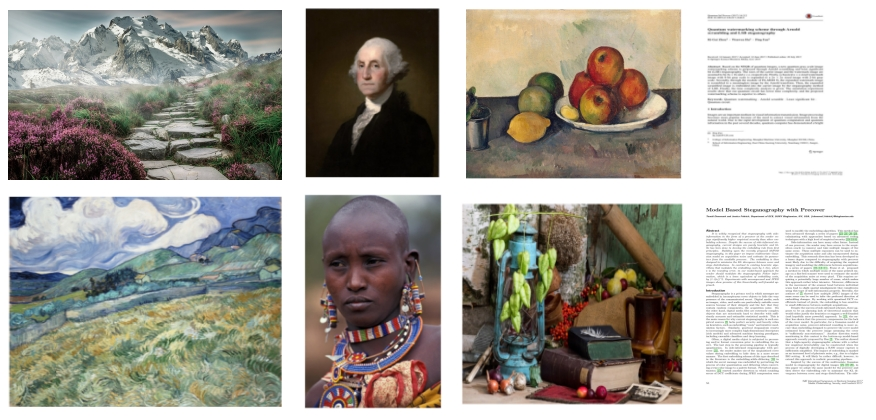
\includegraphics[scale=0.5]{Dataset_example.jpeg}
\caption{Two examples for each type from the built dataset are shown. On first column from left, type N images (landscape) are displayed.
On second column type P (portrait) images are shown. Third and fourth columns shows type S (still life) and type T (text) images respectively. }
\label{Fig:Dataset_example}
\end{figure}



\begin{table}[!h] 
\caption{Dataset features.}
\label{Tab:Features}
\begin{tabular}{lclclclclc}
\hline
\hline 
Feature &  Image type\\
\hline
\midrule
{}       & N (landscapes)   & S (still life)    & P (portrait)   & T (text)\\
mean height [pixels] $\pm$ std  &  600 $\pm$ 100 & 600 $\pm$ 100   & 700 $\pm$ 200  & 1500 $\pm$ 100 \\
mean width [pixels] $\pm$ std   &  900 $\pm$ 200 & 800 $\pm$ 200   & 700 $\pm$ 200  &  1100 $\pm $200 \\
mean size [kBytes] $\pm$ std    &  200 $\pm$ 100 & 150 $\pm$ 70    & 120 $\pm$ 50   &  300 $\pm$ 100\\
\hline
\end{tabular}
\end{table}

% 
% \begin{figure}
% \centering
% \begin{tabular}{|c|c|}
% \hline
% \subf{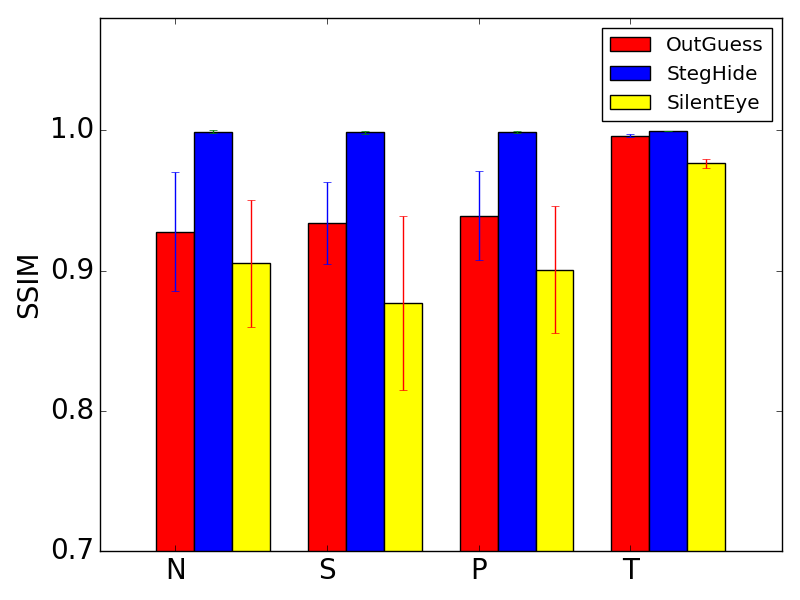
\includegraphics[width=60mm]{SSIM.png}}
% %      {``iteraciones máximas \\ de BT''$=20$}
% &
% \subf{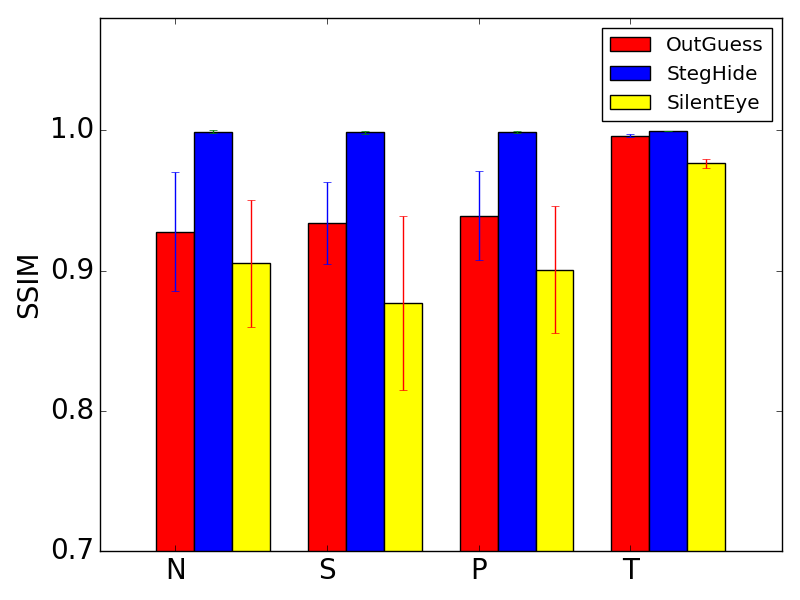
\includegraphics[width=60mm]{SSIM.png}}
% %      {``Periodo de Tenencia \\ en Lista Tabú''$=2$}
% \\
% \hline
% \subf{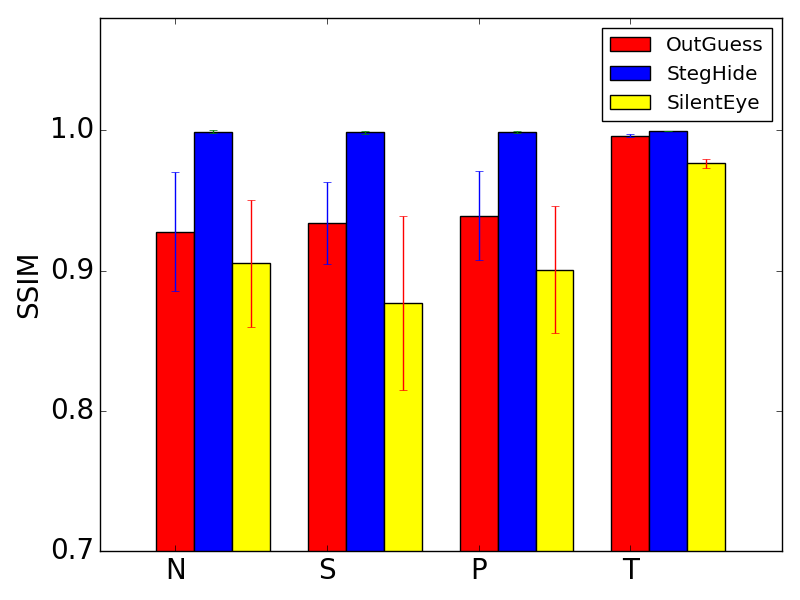
\includegraphics[width=60mm]{SSIM.png}}
% %      {``iteraciones máximas \\ de BT''$=20$}
% &
% \subf{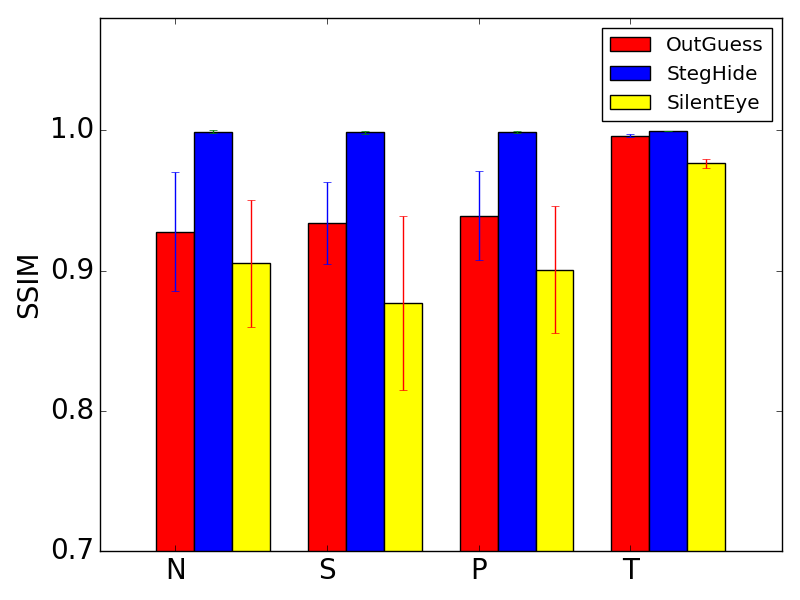
\includegraphics[width=60mm]{SSIM.png}}
% %      {``Periodo de Tenencia \\ en Lista Tabú''$=2$}
% \\
% \hline
% \end{tabular}
% \end{figure}

%Briefing of features for selected softwares
\subsection{Description of selected software}

\subsubsection{\textit{OutGuess (v. 0.2)}}
\textit{OutGuess} is a universal steganographic tool that allows the insertion of hidden information into the  
redundant  bits of data sources. The nature of the data source is irrelevant to the core of \textit{OutGuess}.  The program relies on  
data specific handlers that will extract redundant bits and write them back after modification. Currently only the PPM, 
PNM, and JPEG image formats are supported, although \textit{OutGuess} could use  any  kind  of data, as long as a handler were provided.
\textit{OutGuess} uses  a  generic  iterator  object  to  select  which bits in the data should be modified. A seed can be used 
to modify the behavior of the iterator. It is embedded in the data along with the rest of the message.  
By altering the seed, \textit{OutGuess} tries to find a sequence of bits that minimizes the number of changes in the data that have to be 
made. \textit A bias is introduced that favors the modification of bits that were extracted from a high value, and tries to avoid the 
modification of bits that were extracted from a low value.
Additionally, \textit{OutGuess}  allows  for the hiding of two distinct messages in the data, thus providing plausible 
deniablity.  It keeps track of the bits that have been modified previously and locks them. A (23,12,7)  Golay  code  
is used for error correction to tolerate collisions on locked bits.  Artificial errors are introduced to avoid modifying bits 
that have a high bias.

% \subsubsection{\textit{}}

\subsubsection{\textit{StegHide (v. 0.5.1)}}
\textit{StegHide} is an open source steganographic software that allows hide text using image or sound files as covers. 
It supports JPEG, BMP, WAV and AU file formats as cover files. 
\textit{StegHide} performs steganography by means of a graph-theoretic approach. Data to be embedded is compressed and encrypted,
Then a pseudo-random sequence of postions of pixels is created. On this positions secret data will be embedded. Then a
graph-theoretic  matching  algorithm finds pairs of positions on the remaining pixels such that exchanging their values has
the effect of embedding the corresponding  part of the secret data. If there are not enough pixels with values that can be used
to embed the data by exchanging, values are overwroute. This way, most of the embedding  is  done  by  exchanging  pixel  values
and then the first-order statistics is marginally changed. A passphrase must be provided by the user for encryption and
pseudo-random generator initialization. The same passphrase must be provided for data extraction from stego-file. The default
encryption algorithm is Rijndael with a key of 128 bits altough others are available as well.




\subsubsection{\textit{SilentEye}}
\textit{SilentEye} is a cross-platform steganographic software that allows to hide messages into pictures or sounds. It is free and it is open source. It can be used in Microsoft Windows, Mac OS X and Linux. \\
This software supports JPEG, BMP and WAVE format cover files. It provides too, with all its versions, a simple graphical interface and from version 4.4 the option to be used through the command line. \\
In \textit{SilentEye} you can drag and drop to encode and decode data. The encoding window allows you to choose encoding format, output image’s quality and other settings. You can have a .txt or any other file ready and merge it directly with the cover file or write a message directly into the program in order to hide it inside the file.\\
This tool informs us the number of bytes available to hide in the selected cover image.
\textit{SilentEye} also can encrypt the message before hide it into the cover file. 

% \subsubsection{\textit{SteganPEG}}

%Imperceptibility, capacity and robustness assessment
\subsection{Benchmarking}

Some criteria and metrics needs to be established in order to to benchmark the selected software.
In this section metrics for imperceptibility assessment are presented as well as criteria regarding capacity of storage for
hidden data and tests for robustness evaluation.

\subsubsection{Imperceptibility}

Imperceptibility is a measure of how much the stego-file
looks like the original cover file. Is a critical attribute of a steganography system. Having a poor imperceptibility level will make it 
easier for an eavesdropper to detect the presence of a secret message. For imperceptibility assessment we have selected
two widely known metrics namely, Peak Signal to Noise Ratio (PSNR) and Structural Similarity (SSIM) \cite{Rabie-2019}.

\subsubsection{Capacity}

Capacity refers to the size of the hidden secret data that a steganographic system is able to embed into to the cover
medium. Capacity of a steganographic system depends on the method used to hide data. Hence, different systems can embed
different amount of data given the same cover. Capacity for digital image-based steganograpy can be computed as 
(PONER ECUACIÓN) [REF]


\subsubsection{Robustness}
\label{Subsubsec:Robustness}

Robustness of a steganographic medium is the property of keep the secret information undestroyed under transformation or 
tampering of the stego-file. Sistematic assessment of robustness can be done by applying known transformations to the stego-file
and evaluating the quality of the hidden data recovered from it. In this work robustness for each steganograpic tool 
was tested under five tampering scenarios: overwriting of 10\% of pixels to zero; add of gaussian noise with $\mu = 0$ and $\sigma^2 = 2.5\ 10^{-3}$; horizontal
stretching by 30\%; vertical mirroring; and 20$^o$ counter clock-wise rotation.


\section{Results}


%Show imperceptibility, capacity and robustness results
\subsection{Imperceptibility}

In Figure \ref{Fig:PSNR} and Figure \ref{Fig:SSIM} results for PSNR and SSIM are respectively shown.

\begin{figure}[h!]
\centering
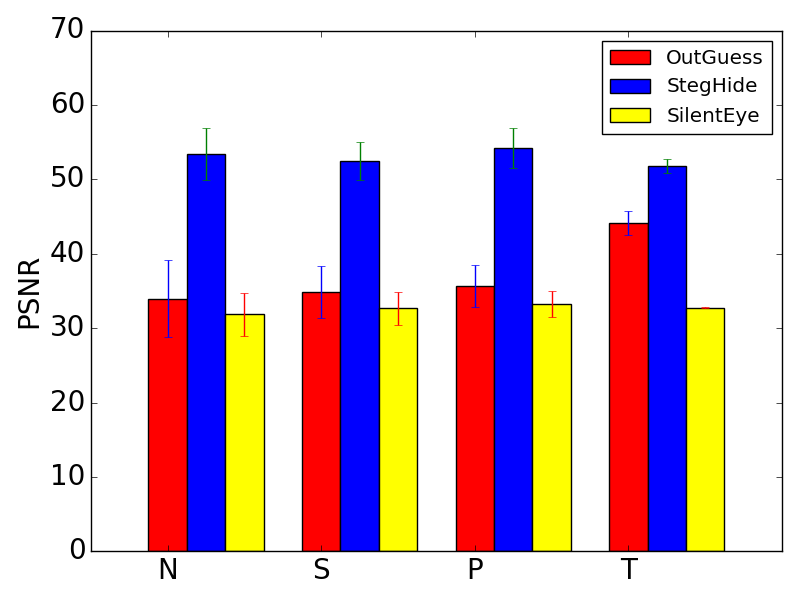
\includegraphics[scale=0.4]{PSNR.png}
\caption{Peak Signal to Noise Ratio for each software and each image type.}
\label{Fig:PSNR}
\end{figure}

\begin{figure}[h!]
\centering
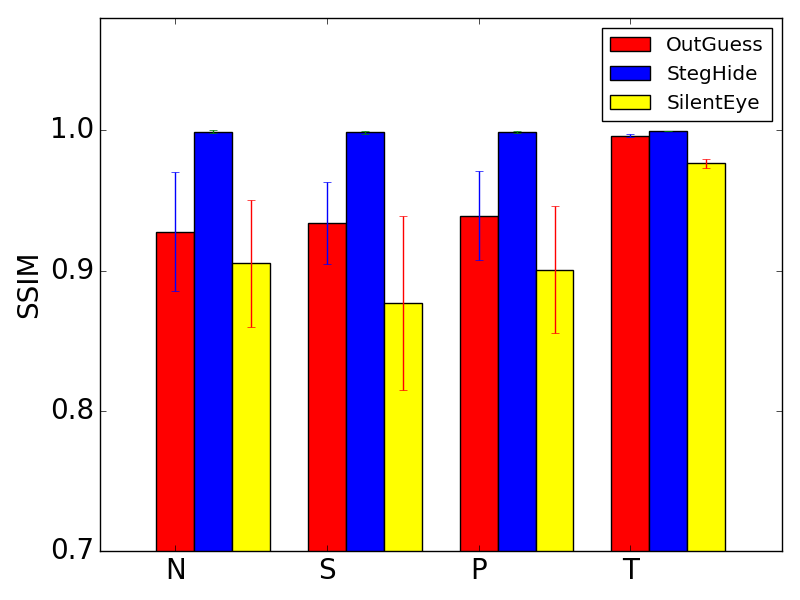
\includegraphics[scale=0.4]{SSIM.png}
\caption{Structural Similarity for each software and each image type.}
\label{Fig:SSIM}
\end{figure}

\subsection{Capacity}

Each software provides an option to evaluate the capacity for a given image. For the dataset used, capacity was obtained
relative to each image size and the mean was computed. Results are shown in Table \ref{Tab:Capacity}.


\begin{table}[!h] 
\caption{Capcity results for each software.}
\label{Tab:Capacity}
\begin{tabular}{lclc}
\hline
\hline 
Software &  Capacity per kBytes of cover image [kBytes] \\
\hline
\midrule
{}       &   \\
OutGuess  &  0.10  \\
StegHide  &  0.05 \\
SilentEye   &  0.01 \\
\hline
\end{tabular}
\end{table}


\subsection{Robustness}

None of the three softwares have shown robustness at all. Any of the five transformations mentioned on Section 
\ref{Subsubsec:Robustness} made unable to recover the hidden data.

\section{Discussion and Conclusion}
All the tested software performed remarkably differently in terms of the type of image in which they hid the text. StegHide had 
the best overall performance except for text images, where each had a similar performance.
It is striking that no software was robust in preserving the integrity of the hidden text, after altering the image in small 
proportions.
Even taking into account that we stayed within the base parameters (limit of the length of the text in bytes per byte of the 
image in which to hide said text) established by each of the proven steganography software.
However, we tried to substantially reduce the length of the text to be hidden below the limits established by each software and 
we found that in the case of OutGuess, reducing the length of the text to be hidden by 80p, it was possible to decode it even 
after having made the alterations previously mentioned.
It would be interesting to find out what is said threshold for each of the software tested and in the future include these 
results in the official bibliography for each software.

% \section{References}

  \begin{thebibliography}{1}

  \bibitem{Shih-Book} F. Shih {\em Digital Watermarking and Steganography: Fundamentals and Techniques
(Second Edition)} 2017. CRC Press.					
  
  \bibitem{Rabie-2019} T. Rabie, M. Baziyad, T. Bonny, R. Fareh {\em Toward a Unified Performance Metric for Benchmarking
Steganography Systems} 2019. Journal of Circuits, Systems and Computers. World Scientific Publishing Company.

%   \bibitem{impj}  The Japan Reader {\em Imperial Japan 1800-1945} 1973:
%   Random House, N.Y.
% 
%   \bibitem{norman} E. H. Norman {\em Japan's emergence as a modern
%   state} 1940: International Secretariat, Institute of Pacific
%   Relations.
% 
%   \bibitem{fo} Bob Tadashi Wakabayashi {\em Anti-Foreignism and Western
%   Learning in Early-Modern Japan} 1986: Harvard University Press.

  \end{thebibliography}


\end{document}
